% Options for packages loaded elsewhere
\PassOptionsToPackage{unicode}{hyperref}
\PassOptionsToPackage{hyphens}{url}
%
\documentclass[
]{article}
\usepackage{lmodern}
\usepackage{amssymb,amsmath}
\usepackage{ifxetex,ifluatex}
\ifnum 0\ifxetex 1\fi\ifluatex 1\fi=0 % if pdftex
  \usepackage[T1]{fontenc}
  \usepackage[utf8]{inputenc}
  \usepackage{textcomp} % provide euro and other symbols
\else % if luatex or xetex
  \usepackage{unicode-math}
  \defaultfontfeatures{Scale=MatchLowercase}
  \defaultfontfeatures[\rmfamily]{Ligatures=TeX,Scale=1}
\fi
% Use upquote if available, for straight quotes in verbatim environments
\IfFileExists{upquote.sty}{\usepackage{upquote}}{}
\IfFileExists{microtype.sty}{% use microtype if available
  \usepackage[]{microtype}
  \UseMicrotypeSet[protrusion]{basicmath} % disable protrusion for tt fonts
}{}
\makeatletter
\@ifundefined{KOMAClassName}{% if non-KOMA class
  \IfFileExists{parskip.sty}{%
    \usepackage{parskip}
  }{% else
    \setlength{\parindent}{0pt}
    \setlength{\parskip}{6pt plus 2pt minus 1pt}}
}{% if KOMA class
  \KOMAoptions{parskip=half}}
\makeatother
\usepackage{xcolor}
\IfFileExists{xurl.sty}{\usepackage{xurl}}{} % add URL line breaks if available
\IfFileExists{bookmark.sty}{\usepackage{bookmark}}{\usepackage{hyperref}}
\hypersetup{
  pdftitle={Econometrics II - Problem 4},
  pdfauthor={William Radaic Peron},
  hidelinks,
  pdfcreator={LaTeX via pandoc}}
\urlstyle{same} % disable monospaced font for URLs
\usepackage[margin=1in]{geometry}
\usepackage{color}
\usepackage{fancyvrb}
\newcommand{\VerbBar}{|}
\newcommand{\VERB}{\Verb[commandchars=\\\{\}]}
\DefineVerbatimEnvironment{Highlighting}{Verbatim}{commandchars=\\\{\}}
% Add ',fontsize=\small' for more characters per line
\usepackage{framed}
\definecolor{shadecolor}{RGB}{248,248,248}
\newenvironment{Shaded}{\begin{snugshade}}{\end{snugshade}}
\newcommand{\AlertTok}[1]{\textcolor[rgb]{0.94,0.16,0.16}{#1}}
\newcommand{\AnnotationTok}[1]{\textcolor[rgb]{0.56,0.35,0.01}{\textbf{\textit{#1}}}}
\newcommand{\AttributeTok}[1]{\textcolor[rgb]{0.77,0.63,0.00}{#1}}
\newcommand{\BaseNTok}[1]{\textcolor[rgb]{0.00,0.00,0.81}{#1}}
\newcommand{\BuiltInTok}[1]{#1}
\newcommand{\CharTok}[1]{\textcolor[rgb]{0.31,0.60,0.02}{#1}}
\newcommand{\CommentTok}[1]{\textcolor[rgb]{0.56,0.35,0.01}{\textit{#1}}}
\newcommand{\CommentVarTok}[1]{\textcolor[rgb]{0.56,0.35,0.01}{\textbf{\textit{#1}}}}
\newcommand{\ConstantTok}[1]{\textcolor[rgb]{0.00,0.00,0.00}{#1}}
\newcommand{\ControlFlowTok}[1]{\textcolor[rgb]{0.13,0.29,0.53}{\textbf{#1}}}
\newcommand{\DataTypeTok}[1]{\textcolor[rgb]{0.13,0.29,0.53}{#1}}
\newcommand{\DecValTok}[1]{\textcolor[rgb]{0.00,0.00,0.81}{#1}}
\newcommand{\DocumentationTok}[1]{\textcolor[rgb]{0.56,0.35,0.01}{\textbf{\textit{#1}}}}
\newcommand{\ErrorTok}[1]{\textcolor[rgb]{0.64,0.00,0.00}{\textbf{#1}}}
\newcommand{\ExtensionTok}[1]{#1}
\newcommand{\FloatTok}[1]{\textcolor[rgb]{0.00,0.00,0.81}{#1}}
\newcommand{\FunctionTok}[1]{\textcolor[rgb]{0.00,0.00,0.00}{#1}}
\newcommand{\ImportTok}[1]{#1}
\newcommand{\InformationTok}[1]{\textcolor[rgb]{0.56,0.35,0.01}{\textbf{\textit{#1}}}}
\newcommand{\KeywordTok}[1]{\textcolor[rgb]{0.13,0.29,0.53}{\textbf{#1}}}
\newcommand{\NormalTok}[1]{#1}
\newcommand{\OperatorTok}[1]{\textcolor[rgb]{0.81,0.36,0.00}{\textbf{#1}}}
\newcommand{\OtherTok}[1]{\textcolor[rgb]{0.56,0.35,0.01}{#1}}
\newcommand{\PreprocessorTok}[1]{\textcolor[rgb]{0.56,0.35,0.01}{\textit{#1}}}
\newcommand{\RegionMarkerTok}[1]{#1}
\newcommand{\SpecialCharTok}[1]{\textcolor[rgb]{0.00,0.00,0.00}{#1}}
\newcommand{\SpecialStringTok}[1]{\textcolor[rgb]{0.31,0.60,0.02}{#1}}
\newcommand{\StringTok}[1]{\textcolor[rgb]{0.31,0.60,0.02}{#1}}
\newcommand{\VariableTok}[1]{\textcolor[rgb]{0.00,0.00,0.00}{#1}}
\newcommand{\VerbatimStringTok}[1]{\textcolor[rgb]{0.31,0.60,0.02}{#1}}
\newcommand{\WarningTok}[1]{\textcolor[rgb]{0.56,0.35,0.01}{\textbf{\textit{#1}}}}
\usepackage{graphicx,grffile}
\makeatletter
\def\maxwidth{\ifdim\Gin@nat@width>\linewidth\linewidth\else\Gin@nat@width\fi}
\def\maxheight{\ifdim\Gin@nat@height>\textheight\textheight\else\Gin@nat@height\fi}
\makeatother
% Scale images if necessary, so that they will not overflow the page
% margins by default, and it is still possible to overwrite the defaults
% using explicit options in \includegraphics[width, height, ...]{}
\setkeys{Gin}{width=\maxwidth,height=\maxheight,keepaspectratio}
% Set default figure placement to htbp
\makeatletter
\def\fps@figure{htbp}
\makeatother
\setlength{\emergencystretch}{3em} % prevent overfull lines
\providecommand{\tightlist}{%
  \setlength{\itemsep}{0pt}\setlength{\parskip}{0pt}}
\setcounter{secnumdepth}{-\maxdimen} % remove section numbering

\title{Econometrics II - Problem 4}
\author{William Radaic Peron}
\date{\today}

\begin{document}
\maketitle

In this problem, we'll be tackling the issue of \emph{forecasting} of an
ARMA model. The problem is split in two parts: (i)
\emph{cross-validation}; and (ii) \emph{bootstrapping}.

\section{Identification and estimation}

First, let's identify the best model for our time series.

\begin{Shaded}
\begin{Highlighting}[]
\NormalTok{df <-}\StringTok{ }\KeywordTok{data.frame}\NormalTok{(df)}

\NormalTok{pplot <-}\StringTok{ }\KeywordTok{ggplot}\NormalTok{(}\DataTypeTok{data =}\NormalTok{ df, }\KeywordTok{aes}\NormalTok{(}\DataTypeTok{x =}\NormalTok{ t, }\DataTypeTok{y =}\NormalTok{ value)) }\OperatorTok{+}\StringTok{ }\KeywordTok{geom_line}\NormalTok{() }\OperatorTok{+}\StringTok{ }
\StringTok{    }\KeywordTok{ggtitle}\NormalTok{(}\StringTok{"Time series plot"}\NormalTok{) }\OperatorTok{+}\StringTok{ }\KeywordTok{theme_few}\NormalTok{()}
\NormalTok{pplot}
\end{Highlighting}
\end{Shaded}

\begin{center}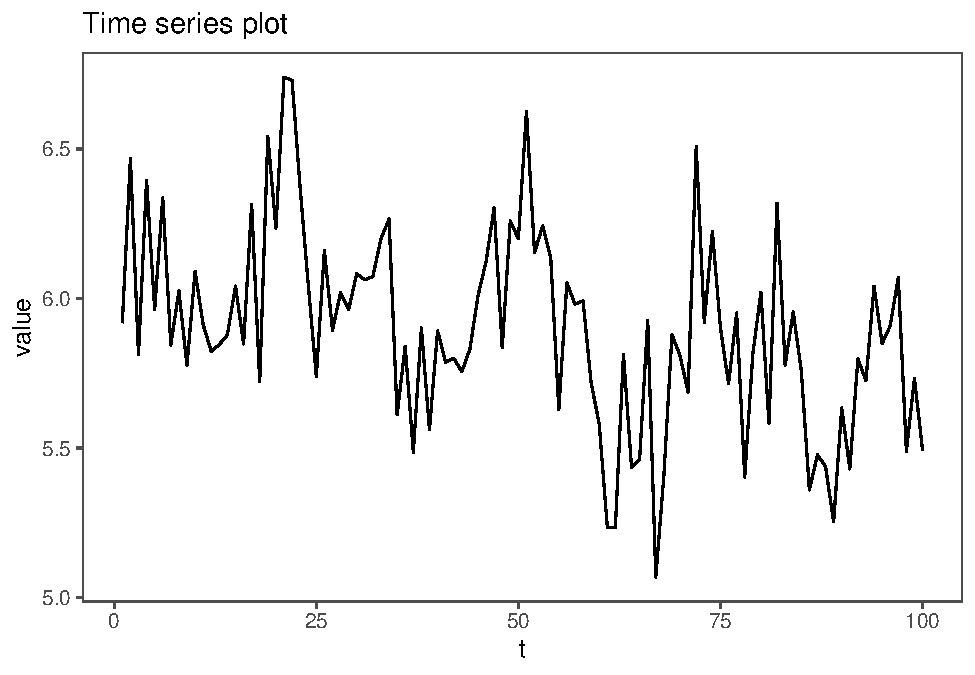
\includegraphics{Econo2_P4_files/figure-latex/plots-1} \end{center}

\begin{Shaded}
\begin{Highlighting}[]
\NormalTok{acf_ts <-}\StringTok{ }\KeywordTok{Acf}\NormalTok{(df}\OperatorTok{$}\NormalTok{value, }\DataTypeTok{lag.max =} \DecValTok{5000}\NormalTok{)}
\end{Highlighting}
\end{Shaded}

\begin{center}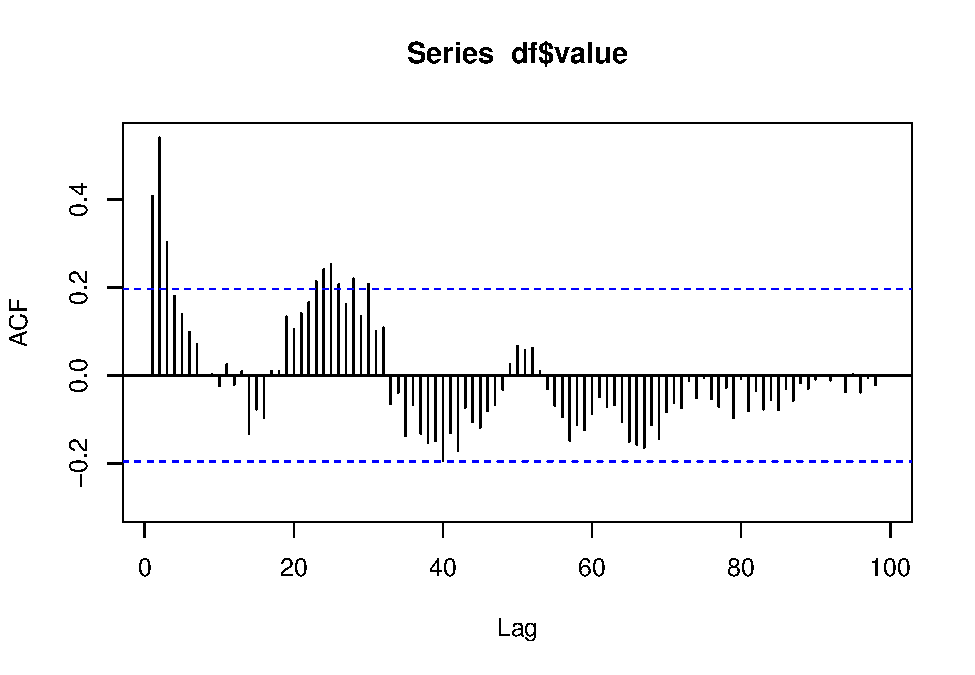
\includegraphics{Econo2_P4_files/figure-latex/plots-2} \end{center}

\begin{Shaded}
\begin{Highlighting}[]
\NormalTok{acf_test_values <-}\StringTok{ }\NormalTok{acf_ts}\OperatorTok{$}\NormalTok{acf}\OperatorTok{/}\KeywordTok{sd}\NormalTok{(acf_ts}\OperatorTok{$}\NormalTok{acf)}

\KeywordTok{head}\NormalTok{(}\KeywordTok{data.frame}\NormalTok{(acf_test_values))}
\end{Highlighting}
\end{Shaded}

\begin{verbatim}
##   acf_test_values
## 1        6.176432
## 2        2.515951
## 3        3.335438
## 4        1.864909
## 5        1.112884
## 6        0.858639
\end{verbatim}

\begin{Shaded}
\begin{Highlighting}[]
\NormalTok{facst <-}\StringTok{ }\KeywordTok{ggAcf}\NormalTok{(df}\OperatorTok{$}\NormalTok{value, }\DataTypeTok{type =} \StringTok{"correlation"}\NormalTok{, }\DataTypeTok{lag.max =} \DecValTok{20}\NormalTok{, }
    \DataTypeTok{plot =}\NormalTok{ T) }\OperatorTok{+}\StringTok{ }\KeywordTok{theme_few}\NormalTok{()}
\NormalTok{faclt <-}\StringTok{ }\KeywordTok{ggAcf}\NormalTok{(df}\OperatorTok{$}\NormalTok{value, }\DataTypeTok{type =} \StringTok{"correlation"}\NormalTok{, }\DataTypeTok{lag.max =} \DecValTok{5000}\NormalTok{, }
    \DataTypeTok{plot =}\NormalTok{ T) }\OperatorTok{+}\StringTok{ }\KeywordTok{theme_few}\NormalTok{()}

\NormalTok{facpst <-}\StringTok{ }\KeywordTok{ggPacf}\NormalTok{(df}\OperatorTok{$}\NormalTok{value, }\DataTypeTok{type =} \StringTok{"correlation"}\NormalTok{, }\DataTypeTok{lag.max =} \DecValTok{100}\NormalTok{, }
    \DataTypeTok{plot =}\NormalTok{ T) }\OperatorTok{+}\StringTok{ }\KeywordTok{theme_few}\NormalTok{()}
\end{Highlighting}
\end{Shaded}

\begin{verbatim}
## Warning: Ignoring unknown parameters: type
\end{verbatim}

\begin{Shaded}
\begin{Highlighting}[]
\NormalTok{facplt <-}\StringTok{ }\KeywordTok{ggPacf}\NormalTok{(df}\OperatorTok{$}\NormalTok{value, }\DataTypeTok{type =} \StringTok{"correlation"}\NormalTok{, }\DataTypeTok{lag.max =} \DecValTok{5000}\NormalTok{, }
    \DataTypeTok{plot =}\NormalTok{ T) }\OperatorTok{+}\StringTok{ }\KeywordTok{theme_few}\NormalTok{()}
\end{Highlighting}
\end{Shaded}

\begin{verbatim}
## Warning: Ignoring unknown parameters: type
\end{verbatim}

\begin{Shaded}
\begin{Highlighting}[]
\NormalTok{facst}
\end{Highlighting}
\end{Shaded}

\begin{center}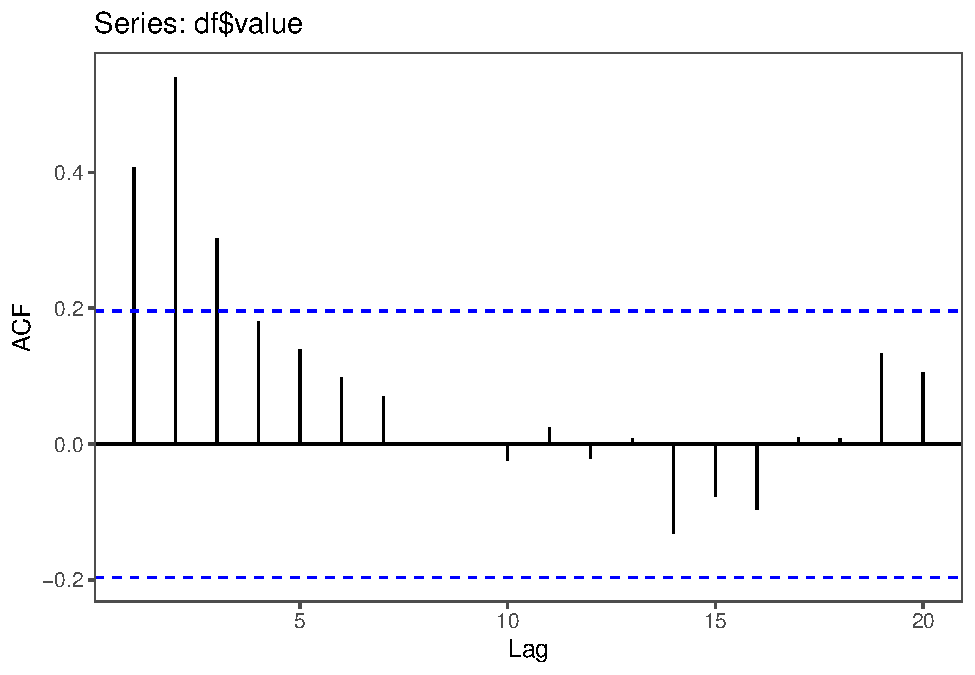
\includegraphics{Econo2_P4_files/figure-latex/plots-3} \end{center}

\begin{Shaded}
\begin{Highlighting}[]
\NormalTok{faclt}
\end{Highlighting}
\end{Shaded}

\begin{center}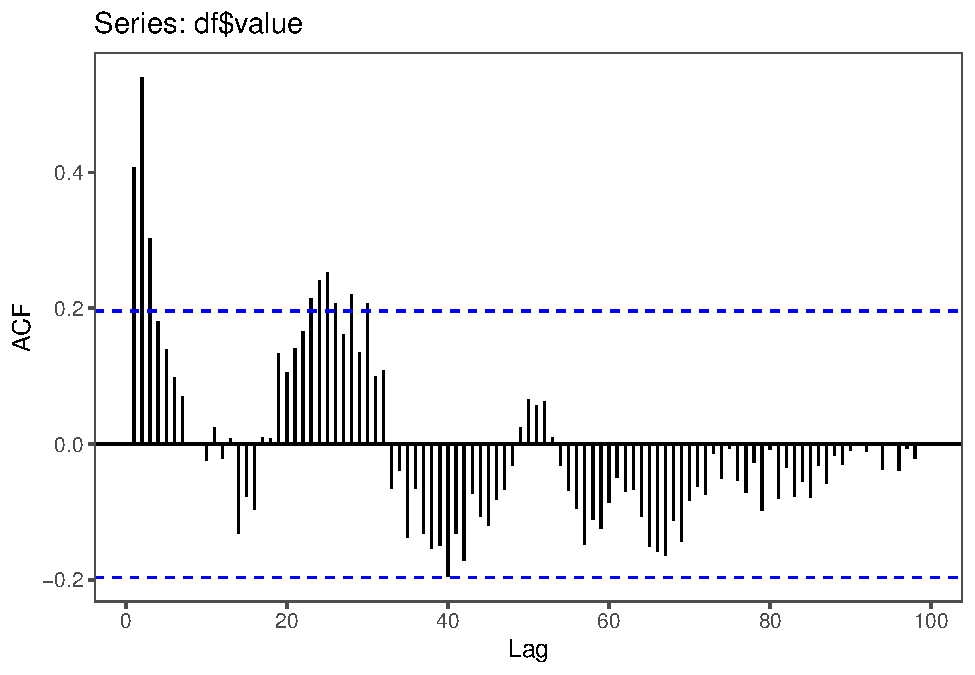
\includegraphics{Econo2_P4_files/figure-latex/plots-4} \end{center}

\begin{Shaded}
\begin{Highlighting}[]
\NormalTok{facpst}
\end{Highlighting}
\end{Shaded}

\begin{center}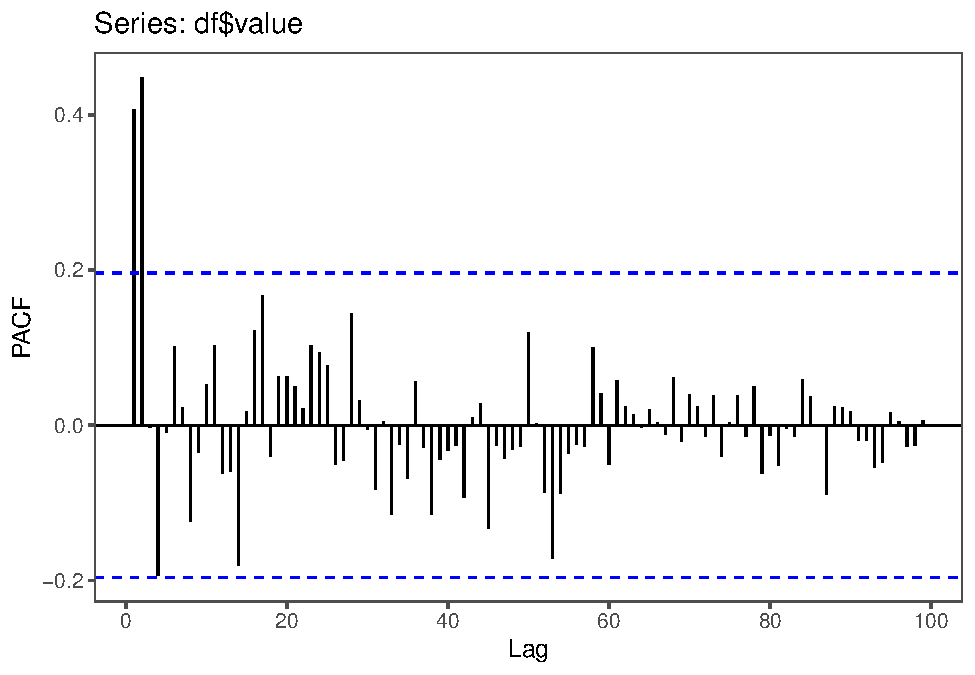
\includegraphics{Econo2_P4_files/figure-latex/plots-5} \end{center}

\begin{Shaded}
\begin{Highlighting}[]
\NormalTok{facplt}
\end{Highlighting}
\end{Shaded}

\begin{center}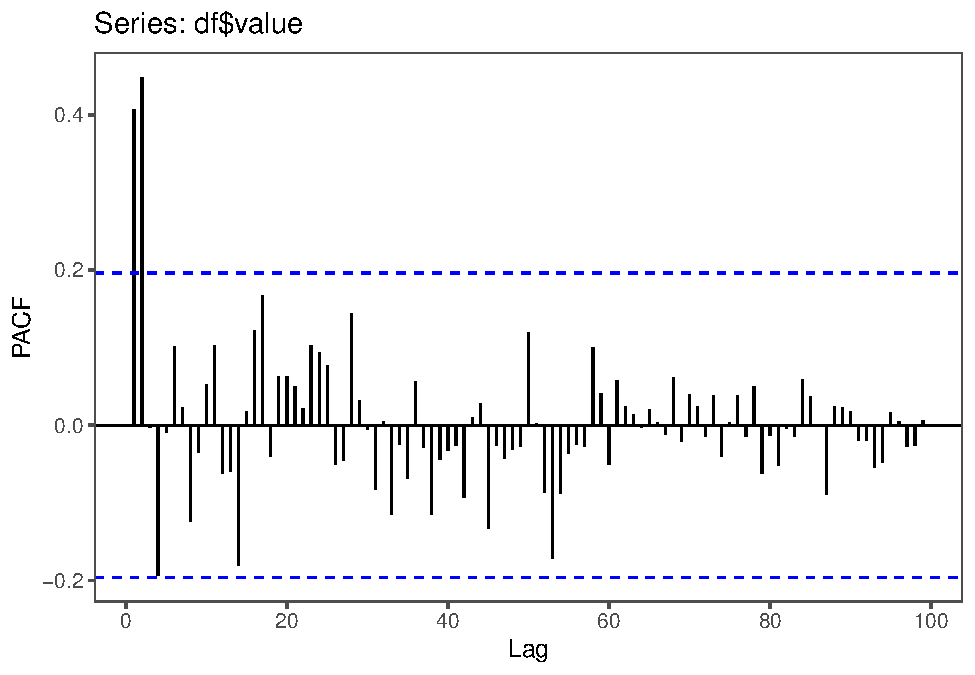
\includegraphics{Econo2_P4_files/figure-latex/plots-6} \end{center}

We'll now use the function \emph{auto.arima} from the package
\emph{forecast} to identify and estimate the model.

\begin{Shaded}
\begin{Highlighting}[]
\NormalTok{aa_model <-}\StringTok{ }\KeywordTok{auto.arima}\NormalTok{(df}\OperatorTok{$}\NormalTok{value, }\DataTypeTok{num.cores =} \DecValTok{24}\NormalTok{, }\DataTypeTok{max.d =} \DecValTok{0}\NormalTok{, }\DataTypeTok{stepwise =}\NormalTok{ F)}

\KeywordTok{summary}\NormalTok{(aa_model)}
\end{Highlighting}
\end{Shaded}

\begin{verbatim}
## Series: df$value 
## ARIMA(0,0,3) with non-zero mean 
## 
## Coefficients:
##          ma1     ma2     ma3    mean
##       0.1814  0.6647  0.4001  5.8982
## s.e.  0.0852  0.0750  0.0949  0.0562
## 
## sigma^2 estimated as 0.0667:  log likelihood=-5.42
## AIC=20.85   AICc=21.49   BIC=33.88
## 
## Training set error measures:
##                        ME      RMSE       MAE        MPE     MAPE      MASE
## Training set -0.002315954 0.2530428 0.2131067 -0.2268814 3.612855 0.7314965
##                    ACF1
## Training set 0.03868106
\end{verbatim}

\begin{Shaded}
\begin{Highlighting}[]
\KeywordTok{print}\NormalTok{(}\StringTok{"t-values: "}\NormalTok{)}
\end{Highlighting}
\end{Shaded}

\begin{verbatim}
## [1] "t-values: "
\end{verbatim}

\begin{Shaded}
\begin{Highlighting}[]
\NormalTok{aa_t <-}\StringTok{ }\KeywordTok{matrix}\NormalTok{(}\OtherTok{NA}\NormalTok{, }\DataTypeTok{nrow =}\NormalTok{ aa_model}\OperatorTok{$}\NormalTok{arma[}\DecValTok{1}\NormalTok{] }\OperatorTok{+}\StringTok{ }\NormalTok{aa_model}\OperatorTok{$}\NormalTok{arma[}\DecValTok{2}\NormalTok{])}

\ControlFlowTok{for}\NormalTok{ (i }\ControlFlowTok{in} \KeywordTok{c}\NormalTok{(}\DecValTok{1}\OperatorTok{:}\DecValTok{4}\NormalTok{)) \{}
    
\NormalTok{    aa_t[i] <-}\StringTok{ }\NormalTok{aa_model}\OperatorTok{$}\NormalTok{coef[i]}\OperatorTok{/}\KeywordTok{sqrt}\NormalTok{(aa_model}\OperatorTok{$}\NormalTok{var.coef[i, i])}
    
\NormalTok{\}}

\NormalTok{aa_t <-}\StringTok{ }\KeywordTok{data.frame}\NormalTok{(aa_t)}

\NormalTok{aa_t}
\end{Highlighting}
\end{Shaded}

\begin{verbatim}
##         aa_t
## 1   2.128691
## 2   8.861580
## 3   4.216481
## 4 105.004537
\end{verbatim}

\begin{Shaded}
\begin{Highlighting}[]
\NormalTok{aa_q <-}\StringTok{ }\KeywordTok{Box.test}\NormalTok{(aa_model}\OperatorTok{$}\NormalTok{residuals, }\DataTypeTok{lag =}\NormalTok{ aa_model}\OperatorTok{$}\NormalTok{arma[}\DecValTok{1}\NormalTok{] }\OperatorTok{+}\StringTok{ }
\StringTok{    }\NormalTok{aa_model}\OperatorTok{$}\NormalTok{arma[}\DecValTok{2}\NormalTok{])}
\NormalTok{aa_q}
\end{Highlighting}
\end{Shaded}

\begin{verbatim}
## 
##  Box-Pierce test
## 
## data:  aa_model$residuals
## X-squared = 0.35002, df = 3, p-value = 0.9504
\end{verbatim}

\begin{Shaded}
\begin{Highlighting}[]
\NormalTok{criteria <-}\StringTok{ }\KeywordTok{matrix}\NormalTok{(}\OtherTok{NA}\NormalTok{, }\DataTypeTok{nrow =} \DecValTok{1}\NormalTok{, }\DataTypeTok{ncol =} \DecValTok{3}\NormalTok{)}

\NormalTok{aa_criteria <-}\StringTok{ }\KeywordTok{data.frame}\NormalTok{(}\StringTok{"MA(3)*"}\NormalTok{, aa_model}\OperatorTok{$}\NormalTok{aic, aa_model}\OperatorTok{$}\NormalTok{bic)}

\KeywordTok{names}\NormalTok{(aa_criteria) <-}\StringTok{ }\KeywordTok{c}\NormalTok{(}\StringTok{"Model"}\NormalTok{, }\StringTok{"AIC"}\NormalTok{, }\StringTok{"BIC"}\NormalTok{)}

\NormalTok{aa_criteria}
\end{Highlighting}
\end{Shaded}

\begin{verbatim}
##    Model      AIC      BIC
## 1 MA(3)* 20.84963 33.87549
\end{verbatim}

\begin{Shaded}
\begin{Highlighting}[]
\NormalTok{fac_e <-}\StringTok{ }\KeywordTok{ggAcf}\NormalTok{(aa_model}\OperatorTok{$}\NormalTok{residuals, }\DataTypeTok{type =} \StringTok{"correlation"}\NormalTok{, }\DataTypeTok{lag.max =} \DecValTok{20}\NormalTok{, }
    \DataTypeTok{plot =}\NormalTok{ T) }\OperatorTok{+}\StringTok{ }\KeywordTok{theme_few}\NormalTok{()}

\NormalTok{facp_e <-}\StringTok{ }\KeywordTok{ggPacf}\NormalTok{(aa_model}\OperatorTok{$}\NormalTok{residuals, }\DataTypeTok{type =} \StringTok{"correlation"}\NormalTok{, }\DataTypeTok{lag.max =} \DecValTok{20}\NormalTok{, }
    \DataTypeTok{plot =}\NormalTok{ T) }\OperatorTok{+}\StringTok{ }\KeywordTok{theme_few}\NormalTok{()}
\end{Highlighting}
\end{Shaded}

\begin{verbatim}
## Warning: Ignoring unknown parameters: type
\end{verbatim}

\begin{Shaded}
\begin{Highlighting}[]
\NormalTok{fac_e}
\end{Highlighting}
\end{Shaded}

\begin{center}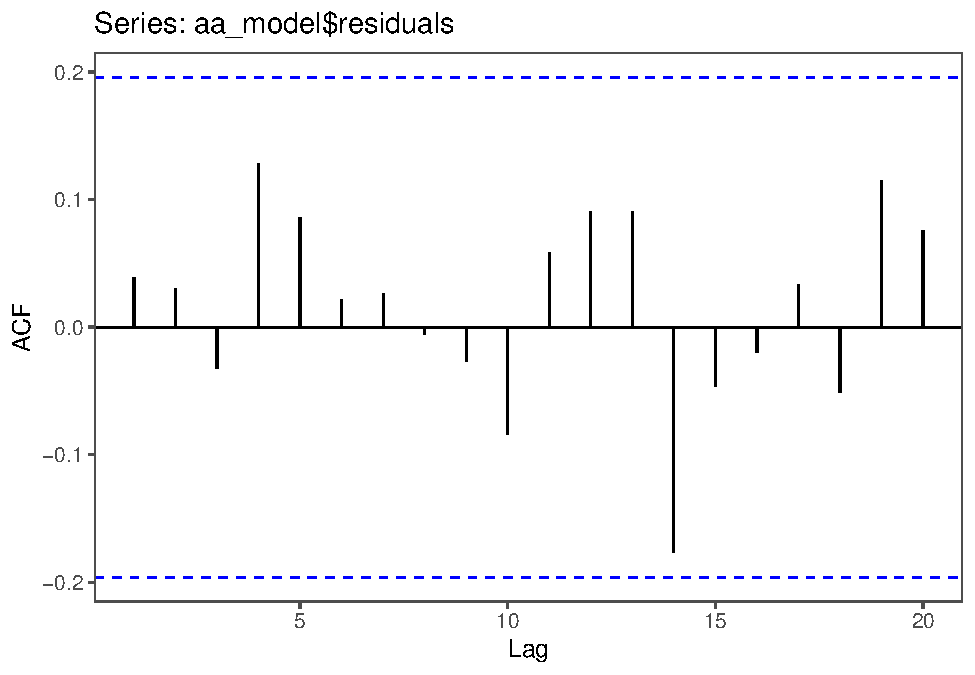
\includegraphics{Econo2_P4_files/figure-latex/estimation autoarima-1} \end{center}

\begin{Shaded}
\begin{Highlighting}[]
\NormalTok{facp_e}
\end{Highlighting}
\end{Shaded}

\begin{center}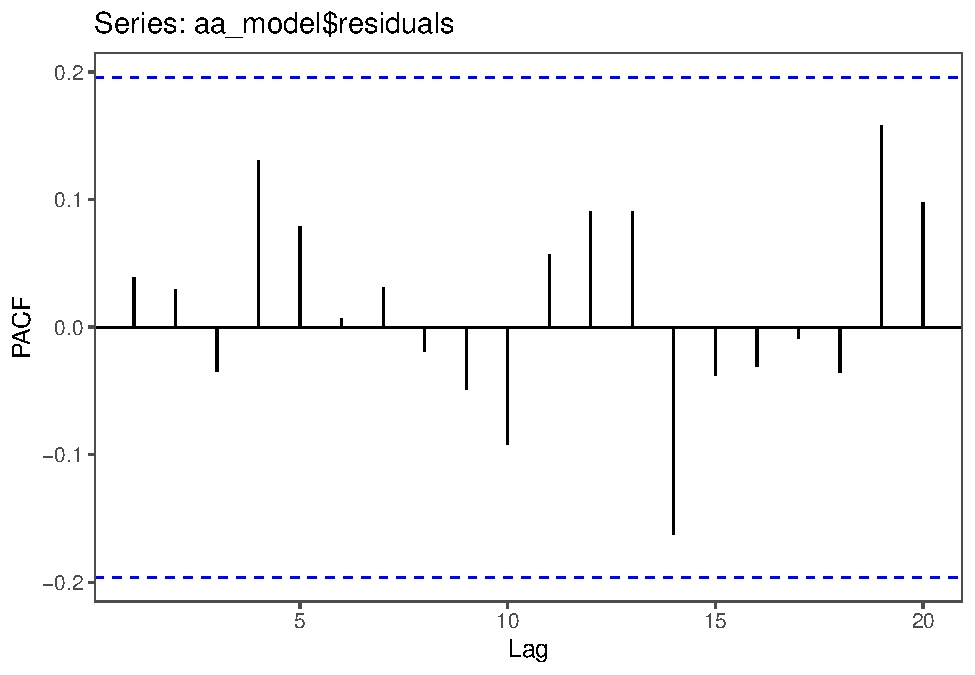
\includegraphics{Econo2_P4_files/figure-latex/estimation autoarima-2} \end{center}

\begin{Shaded}
\begin{Highlighting}[]
\KeywordTok{mean}\NormalTok{(aa_model}\OperatorTok{$}\NormalTok{residuals)}
\end{Highlighting}
\end{Shaded}

\begin{verbatim}
## [1] -0.002315954
\end{verbatim}

The results of \emph{auto.arima} imply that the best model is an
ARMA(0,3) -- i.e., a MA(3):
\[ y_t = c +  + \theta_1 \varepsilon_{t-1} + \theta_2 \varepsilon_{t-2}+ \theta_3 \varepsilon_{t-3} + \varepsilon_t, \hspace{1em} \varepsilon_t \sim wn(0, \sigma^2)\]

Furthermore, the Q-statistic \emph{(Box.test)} seems to indicate that
\(\varepsilon_t\) is truly white noise.

\section{Cross-validation}

Let's now cross-validate or model. This will now be done manually;
afterwards, an automatized version from \emph{fpp} shall be presented.

Let \(h := 5\); \(frac = 0.2\). \(T\) is the size of our sample; \(k\)
is the \emph{training} database. The remainder shall be used for testing
purposes.

As we have discovered previously, \emph{auto.arima} yields a
\textbf{MA(3)} model. It will now be used.

\begin{Shaded}
\begin{Highlighting}[]
\NormalTok{h <-}\StringTok{ }\DecValTok{5}

\NormalTok{frac <-}\StringTok{ }\FloatTok{0.2}

\NormalTok{T <-}\StringTok{ }\KeywordTok{length}\NormalTok{(df}\OperatorTok{$}\NormalTok{value)}

\NormalTok{k <-}\StringTok{ }\KeywordTok{floor}\NormalTok{((}\DecValTok{1} \OperatorTok{-}\StringTok{ }\NormalTok{frac) }\OperatorTok{*}\StringTok{ }\NormalTok{T)}

\CommentTok{# Estimating MA(3) with k = 80}
\NormalTok{fit <-}\StringTok{ }\KeywordTok{Arima}\NormalTok{(df}\OperatorTok{$}\NormalTok{value[}\DecValTok{1}\OperatorTok{:}\NormalTok{k], }\DataTypeTok{order =} \KeywordTok{c}\NormalTok{(}\DecValTok{0}\NormalTok{, }\DecValTok{0}\NormalTok{, }\DecValTok{3}\NormalTok{))}

\CommentTok{# Generating predictions from the model}
\NormalTok{pred <-}\StringTok{ }\KeywordTok{predict}\NormalTok{(fit, }\DataTypeTok{n.ahead =}\NormalTok{ h)}

\CommentTok{# Calculating errors between the predicted values of the}
\CommentTok{# model and the actual values of the testing database}

\NormalTok{e <-}\StringTok{ }\NormalTok{df}\OperatorTok{$}\NormalTok{value[(k }\OperatorTok{+}\StringTok{ }\NormalTok{h)] }\OperatorTok{-}\StringTok{ }\NormalTok{pred}\OperatorTok{$}\NormalTok{pred[h]}

\NormalTok{e}
\end{Highlighting}
\end{Shaded}

\begin{verbatim}
## [1] -0.1951299
\end{verbatim}

Let's now update our training database iteratively with a for loop.

\begin{Shaded}
\begin{Highlighting}[]
\NormalTok{e <-}\StringTok{ }\KeywordTok{matrix}\NormalTok{(}\OtherTok{NA}\NormalTok{, }\DataTypeTok{nrow =} \DecValTok{100}\NormalTok{)}

\CommentTok{# Updating the model}

\ControlFlowTok{for}\NormalTok{ (i }\ControlFlowTok{in}\NormalTok{ k}\OperatorTok{:}\NormalTok{(T }\OperatorTok{-}\StringTok{ }\NormalTok{h)) \{}
    
\NormalTok{    fit <-}\StringTok{ }\KeywordTok{Arima}\NormalTok{(df}\OperatorTok{$}\NormalTok{value[}\DecValTok{1}\OperatorTok{:}\NormalTok{i], }\DataTypeTok{order =} \KeywordTok{c}\NormalTok{(}\DecValTok{0}\NormalTok{, }\DecValTok{0}\NormalTok{, }\DecValTok{3}\NormalTok{))}
    
\NormalTok{    pred <-}\StringTok{ }\KeywordTok{predict}\NormalTok{(fit, }\DataTypeTok{n.ahead =}\NormalTok{ h)}
    
\NormalTok{    e[i, }\DecValTok{1}\NormalTok{] <-}\StringTok{ }\NormalTok{df}\OperatorTok{$}\NormalTok{value[(i }\OperatorTok{+}\StringTok{ }\NormalTok{h)] }\OperatorTok{-}\StringTok{ }\NormalTok{pred}\OperatorTok{$}\NormalTok{pred[h]}
    
\NormalTok{\}}
\end{Highlighting}
\end{Shaded}

With the matrix \emph{e} in hands, we can now calculate MSE:

\begin{Shaded}
\begin{Highlighting}[]
\NormalTok{mse <-}\StringTok{ }\KeywordTok{mean}\NormalTok{(e}\OperatorTok{^}\DecValTok{2}\NormalTok{, }\DataTypeTok{na.rm =}\NormalTok{ T)}
\end{Highlighting}
\end{Shaded}

This procedure can now be used to compare other models against the model
from \emph{auto.arima}.

\begin{Shaded}
\begin{Highlighting}[]
\NormalTok{max_p <-}\StringTok{ }\DecValTok{5}

\NormalTok{max_q <-}\StringTok{ }\DecValTok{5}

\NormalTok{e <-}\StringTok{ }\KeywordTok{matrix}\NormalTok{(}\OtherTok{NA}\NormalTok{, }\DataTypeTok{nrow =} \DecValTok{100}\NormalTok{, }\DataTypeTok{ncol =}\NormalTok{ (max_p }\OperatorTok{+}\StringTok{ }\DecValTok{1}\NormalTok{) }\OperatorTok{*}\StringTok{ }\NormalTok{(max_q }\OperatorTok{+}\StringTok{ }\DecValTok{1}\NormalTok{))}

\NormalTok{pred <-}\StringTok{ }\KeywordTok{vector}\NormalTok{(}\StringTok{"list"}\NormalTok{, (max_p }\OperatorTok{+}\StringTok{ }\DecValTok{1}\NormalTok{) }\OperatorTok{*}\StringTok{ }\NormalTok{(max_q }\OperatorTok{+}\StringTok{ }\DecValTok{1}\NormalTok{))}

\NormalTok{fit <-}\StringTok{ }\KeywordTok{vector}\NormalTok{(}\StringTok{"list"}\NormalTok{, (max_p }\OperatorTok{+}\StringTok{ }\DecValTok{1}\NormalTok{) }\OperatorTok{*}\StringTok{ }\NormalTok{(max_q }\OperatorTok{+}\StringTok{ }\DecValTok{1}\NormalTok{))}

\CommentTok{# Updating the model}
\ControlFlowTok{for}\NormalTok{ (u }\ControlFlowTok{in} \DecValTok{0}\OperatorTok{:}\NormalTok{max_q) \{}
    
    \ControlFlowTok{for}\NormalTok{ (j }\ControlFlowTok{in} \DecValTok{0}\OperatorTok{:}\NormalTok{max_p) \{}
        
        
        \ControlFlowTok{for}\NormalTok{ (i }\ControlFlowTok{in}\NormalTok{ k}\OperatorTok{:}\NormalTok{(T }\OperatorTok{-}\StringTok{ }\NormalTok{h)) \{}
            
\NormalTok{            fit[[(((max_p }\OperatorTok{+}\StringTok{ }\DecValTok{1}\NormalTok{) }\OperatorTok{*}\StringTok{ }\NormalTok{j) }\OperatorTok{+}\StringTok{ }\NormalTok{u }\OperatorTok{+}\StringTok{ }\DecValTok{1}\NormalTok{)]] <-}\StringTok{ }\KeywordTok{Arima}\NormalTok{(df}\OperatorTok{$}\NormalTok{value[}\DecValTok{1}\OperatorTok{:}\NormalTok{i], }
                \DataTypeTok{order =} \KeywordTok{c}\NormalTok{(j, }\DecValTok{0}\NormalTok{, u))}
            
            \CommentTok{# fit <- append(fit, Arima(df$value[1:i], order = c(j,0,u)))}
            
            \CommentTok{# pred <- append(pred, predict(fit[[(j+u)]], n.ahead = h))}
            
\NormalTok{            pred[[(((max_p }\OperatorTok{+}\StringTok{ }\DecValTok{1}\NormalTok{) }\OperatorTok{*}\StringTok{ }\NormalTok{j) }\OperatorTok{+}\StringTok{ }\NormalTok{u }\OperatorTok{+}\StringTok{ }\DecValTok{1}\NormalTok{)]] <-}\StringTok{ }\KeywordTok{predict}\NormalTok{(fit[[(((max_p }\OperatorTok{+}\StringTok{ }
\StringTok{                }\DecValTok{1}\NormalTok{) }\OperatorTok{*}\StringTok{ }\NormalTok{j) }\OperatorTok{+}\StringTok{ }\NormalTok{u }\OperatorTok{+}\StringTok{ }\DecValTok{1}\NormalTok{)]], }\DataTypeTok{n.ahead =}\NormalTok{ h)}
            
\NormalTok{            e[i, (((max_p }\OperatorTok{+}\StringTok{ }\DecValTok{1}\NormalTok{) }\OperatorTok{*}\StringTok{ }\NormalTok{j) }\OperatorTok{+}\StringTok{ }\NormalTok{u }\OperatorTok{+}\StringTok{ }\DecValTok{1}\NormalTok{)] <-}\StringTok{ }\NormalTok{df}\OperatorTok{$}\NormalTok{value[(i }\OperatorTok{+}\StringTok{ }
\StringTok{                }\NormalTok{h)] }\OperatorTok{-}\StringTok{ }\NormalTok{pred[[(((max_p }\OperatorTok{+}\StringTok{ }\DecValTok{1}\NormalTok{) }\OperatorTok{*}\StringTok{ }\NormalTok{j) }\OperatorTok{+}\StringTok{ }\NormalTok{u }\OperatorTok{+}\StringTok{ }\DecValTok{1}\NormalTok{)]]}\OperatorTok{$}\NormalTok{pred[h]}
            
\NormalTok{        \}}
        
\NormalTok{    \}}
    
\NormalTok{\}}

\NormalTok{mse <-}\StringTok{ }\KeywordTok{matrix}\NormalTok{(}\OtherTok{NA}\NormalTok{, }\DataTypeTok{nrow =}\NormalTok{ ((max_p }\OperatorTok{+}\StringTok{ }\DecValTok{1}\NormalTok{) }\OperatorTok{*}\StringTok{ }\NormalTok{(max_q }\OperatorTok{+}\StringTok{ }\DecValTok{1}\NormalTok{)), }\DataTypeTok{ncol =} \DecValTok{1}\NormalTok{)}




\NormalTok{mse <-}\StringTok{ }\KeywordTok{colMeans}\NormalTok{(e}\OperatorTok{^}\DecValTok{2}\NormalTok{, }\DataTypeTok{na.rm =}\NormalTok{ T)}

\NormalTok{mse}
\end{Highlighting}
\end{Shaded}

\begin{verbatim}
##  [1] 0.1357466 0.1354001 0.1368083 0.1374243 0.1376508 0.1441940 0.1347115
##  [8] 0.1269779 0.1347789 0.1373465 0.1398588 0.1436175 0.1313779 0.1315448
## [15] 0.1435805 0.1355649 0.1421277 0.1335153 0.1316765 0.1333955 0.1400838
## [22] 0.1427467 0.1473227 0.1347447 0.1320856 0.1333025 0.1354734 0.1341742
## [29] 0.1380676 0.1357880 0.1346228 0.1382810 0.1319484 0.1308446 0.1382417
## [36] 0.1327046
\end{verbatim}

\begin{Shaded}
\begin{Highlighting}[]
\NormalTok{optimal_index <-}\StringTok{ }\KeywordTok{which.min}\NormalTok{(mse)}

\NormalTok{cv_model <-}\StringTok{ }\NormalTok{fit[[optimal_index]]}

\KeywordTok{summary}\NormalTok{(cv_model)}
\end{Highlighting}
\end{Shaded}

\begin{verbatim}
## Series: df$value[1:i] 
## ARIMA(1,0,1) with non-zero mean 
## 
## Coefficients:
##          ar1      ma1    mean
##       0.8253  -0.4888  5.9125
## s.e.  0.0814   0.1118  0.0815
## 
## sigma^2 estimated as 0.08209:  log likelihood=-14.72
## AIC=37.43   AICc=37.88   BIC=47.65
## 
## Training set error measures:
##                        ME      RMSE       MAE        MPE     MAPE      MASE
## Training set -0.002725722 0.2819456 0.2228183 -0.2756862 3.787114 0.7600473
##                    ACF1
## Training set -0.1279409
\end{verbatim}

The cross-validation method constructed above yielded an ARMA(1,1):
\[ y_t = c + \phi_1 y_{t-1} +  + \theta_1 \varepsilon_{t-1} + \varepsilon_t, \hspace{1em} \varepsilon_t \sim wn(0, \sigma^2)\]

\begin{Shaded}
\begin{Highlighting}[]
\NormalTok{cv_fc <-}\StringTok{ }\KeywordTok{forecast}\NormalTok{(cv_model, }\DataTypeTok{h =}\NormalTok{ h)}

\KeywordTok{autoplot}\NormalTok{(cv_fc)}
\end{Highlighting}
\end{Shaded}

\begin{center}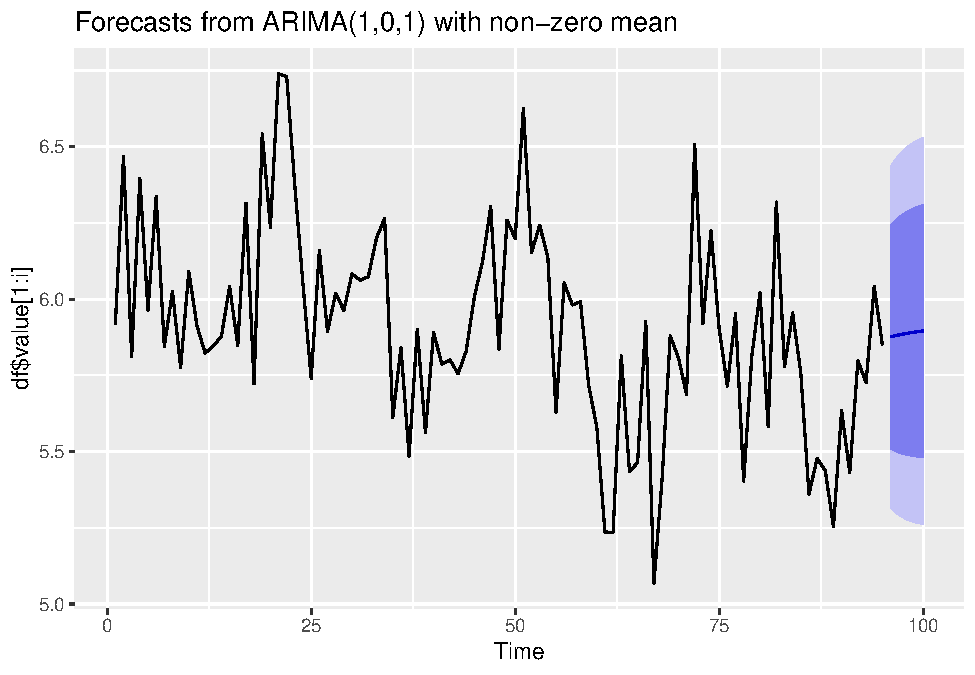
\includegraphics{Econo2_P4_files/figure-latex/forecast cv plot-1} \end{center}

\section{Bootstrapping}

Now, let's proceed to \emph{bootstrapping}. It envolves the following
steps:

\begin{enumerate}
\item \begin{itemize}
\item Estimate ARMA(p,q)
$$ Y_t = c + \sum_{j=1}^p \phi_j Y_{t-j} + \sum_{j=1}^q \theta_j \varepsilon_{t-j} + \varepsilon_t$$

\item Calculate the residuals of the regression:
$$ \hat{\varepsilon}_t := Y_t - (\hat{c} + \sum_{j=1}^p \hat{\phi}_j Y_{t-j} + \sum_{j=1}^q \hat{\theta}_j \varepsilon_{t-j})$$

\item If the residuals do not have mean 0, create the centered residuals:
$$ \tilde{\varepsilon}_t = \hat{\varepsilon}_t - \frac{1}{t} \sum_{t=1}^T \hat{\varepsilon}_t$$
\end{itemize}

\item \begin{itemize}
\item Select at random, with restocking, a sample with $T + m$ elements, $m >> 0$:
$$\{\varepsilon^*_1, ..., \varepsilon^*_{T+m}\}$$
\item Create a series $\{Y^*_t\}_{t=1}^{T+m}$:
$$ Y_t^* = Y_t, 1 \leq t \leq max(p,q) $$
$$ Y_t^* = \hat{c} + \sum_{j=1}^p \hat{\phi}_j Y_{t-j} + \sum_{j=1}^q \hat{\theta}_j \varepsilon_{t-j}^* + \varepsilon_t^*, max(p,q) < t \leq T + m $$
\end{itemize}
\item \begin{itemize}
\item Using the simulated sample $\{Y^*_t\}_{t=1}^{T+m}$, create a forecast for $h >0$ periods using the estimated coefficients *obtained with the real sample*.
\item This yields a vector of dimension $h$ containing the forecasts in the form:
$$(\hat{Y}^*_{T+1}, ..., \hat{Y}^*_{T+h})$$ 
\item Repeat steps 2 and 3 for $S$ times. Create a matrix with the results.

\item This yields a S x h matrix where each row is equal to the aforementioned vector.
\end{itemize}
\end{enumerate}

We'll use, again, the optimal model from \emph{auto.arima}, MA(3):

\[ y_t = c +  + \theta_1 \varepsilon_{t-1} + \theta_2 \varepsilon_{t-2}+ \theta_3 \varepsilon_{t-3} + \varepsilon_t, \hspace{1em} \varepsilon_t \sim wn(0, \sigma^2)\]

\begin{Shaded}
\begin{Highlighting}[]
\NormalTok{S <-}\StringTok{ }\DecValTok{1000}

\NormalTok{m <-}\StringTok{ }\DecValTok{100}



\NormalTok{optimal_p <-}\StringTok{ }\NormalTok{aa_model}\OperatorTok{$}\NormalTok{arma[}\DecValTok{1}\NormalTok{]}

\NormalTok{optimal_q <-}\StringTok{ }\NormalTok{aa_model}\OperatorTok{$}\NormalTok{arma[}\DecValTok{2}\NormalTok{]}

\NormalTok{e_sample <-}\StringTok{ }\KeywordTok{data.frame}\NormalTok{(}\KeywordTok{matrix}\NormalTok{(}\OtherTok{NA}\NormalTok{, }\DataTypeTok{nrow =}\NormalTok{ S, }\DataTypeTok{ncol =}\NormalTok{ (}\KeywordTok{length}\NormalTok{(df}\OperatorTok{$}\NormalTok{value) }\OperatorTok{+}\StringTok{ }
\StringTok{    }\NormalTok{m)))}

\NormalTok{y_star <-}\StringTok{ }\KeywordTok{data.frame}\NormalTok{(}\KeywordTok{matrix}\NormalTok{(}\OtherTok{NA}\NormalTok{, }\DataTypeTok{nrow =}\NormalTok{ S, }\DataTypeTok{ncol =}\NormalTok{ (}\KeywordTok{length}\NormalTok{(df}\OperatorTok{$}\NormalTok{value) }\OperatorTok{+}\StringTok{ }
\StringTok{    }\NormalTok{m }\OperatorTok{+}\StringTok{ }\KeywordTok{max}\NormalTok{(aa_model}\OperatorTok{$}\NormalTok{arma[}\DecValTok{1}\NormalTok{], aa_model}\OperatorTok{$}\NormalTok{arma[}\DecValTok{2}\NormalTok{]))))}

\NormalTok{arima_star <-}\StringTok{ }\KeywordTok{data.frame}\NormalTok{(}\KeywordTok{matrix}\NormalTok{(}\OtherTok{NA}\NormalTok{, }\DataTypeTok{nrow =}\NormalTok{ S, }\DataTypeTok{ncol =}\NormalTok{ (}\KeywordTok{length}\NormalTok{(df}\OperatorTok{$}\NormalTok{value) }\OperatorTok{+}\StringTok{ }
\StringTok{    }\NormalTok{m }\OperatorTok{+}\StringTok{ }\KeywordTok{max}\NormalTok{(aa_model}\OperatorTok{$}\NormalTok{arma[}\DecValTok{1}\NormalTok{], aa_model}\OperatorTok{$}\NormalTok{arma[}\DecValTok{2}\NormalTok{]))))}


\ControlFlowTok{for}\NormalTok{ (i }\ControlFlowTok{in} \DecValTok{1}\OperatorTok{:}\NormalTok{S) \{}
    
\NormalTok{    e_sample[i] <-}\StringTok{ }\KeywordTok{sample}\NormalTok{(aa_model}\OperatorTok{$}\NormalTok{residuals, }\DataTypeTok{replace =}\NormalTok{ T, }\DataTypeTok{size =}\NormalTok{ (}\KeywordTok{length}\NormalTok{(df}\OperatorTok{$}\NormalTok{value) }\OperatorTok{+}\StringTok{ }
\StringTok{        }\NormalTok{m))}
    
\NormalTok{\}}

\ControlFlowTok{for}\NormalTok{ (i }\ControlFlowTok{in} \DecValTok{1}\OperatorTok{:}\NormalTok{S) \{}
    
    \ControlFlowTok{for}\NormalTok{ (j }\ControlFlowTok{in}\NormalTok{ ((aa_model}\OperatorTok{$}\NormalTok{arma[}\DecValTok{1}\NormalTok{] }\OperatorTok{+}\StringTok{ }\NormalTok{aa_model}\OperatorTok{$}\NormalTok{arma[}\DecValTok{2}\NormalTok{] }\OperatorTok{+}\StringTok{ }\DecValTok{1}\NormalTok{)}\OperatorTok{:}\NormalTok{(}\KeywordTok{length}\NormalTok{(df}\OperatorTok{$}\NormalTok{value) }\OperatorTok{+}\StringTok{ }
\StringTok{        }\NormalTok{m))) \{}
        
\NormalTok{        arima_star[i, j] <-}\StringTok{ }\NormalTok{(aa_model}\OperatorTok{$}\NormalTok{coef[}\DecValTok{4}\NormalTok{] }\OperatorTok{+}\StringTok{ }\NormalTok{(aa_model}\OperatorTok{$}\NormalTok{coef[}\DecValTok{1}\NormalTok{] }\OperatorTok{*}\StringTok{ }
\StringTok{            }\NormalTok{e_sample[i, j }\OperatorTok{-}\StringTok{ }\DecValTok{1}\NormalTok{]) }\OperatorTok{+}\StringTok{ }\NormalTok{(aa_model}\OperatorTok{$}\NormalTok{coef[}\DecValTok{2}\NormalTok{] }\OperatorTok{*}\StringTok{ }\NormalTok{e_sample[i, }
\NormalTok{            j }\OperatorTok{-}\StringTok{ }\DecValTok{2}\NormalTok{]) }\OperatorTok{+}\StringTok{ }\NormalTok{(aa_model}\OperatorTok{$}\NormalTok{coef[}\DecValTok{3}\NormalTok{] }\OperatorTok{*}\StringTok{ }\NormalTok{e_sample[i, j }\OperatorTok{-}\StringTok{ }\DecValTok{3}\NormalTok{]) }\OperatorTok{+}\StringTok{ }
\StringTok{            }\NormalTok{e_sample[i, j])}
        
\NormalTok{    \}}
    
\NormalTok{\}}


\NormalTok{y_fixed <-}\StringTok{ }\KeywordTok{data.frame}\NormalTok{(}\KeywordTok{matrix}\NormalTok{(}\OtherTok{NA}\NormalTok{, }\DataTypeTok{nrow =}\NormalTok{ S, }\DataTypeTok{ncol =}\NormalTok{ (aa_model}\OperatorTok{$}\NormalTok{arma[}\DecValTok{1}\NormalTok{] }\OperatorTok{+}\StringTok{ }
\StringTok{    }\NormalTok{aa_model}\OperatorTok{$}\NormalTok{arma[}\DecValTok{2}\NormalTok{])))}

\ControlFlowTok{for}\NormalTok{ (i }\ControlFlowTok{in} \DecValTok{1}\OperatorTok{:}\NormalTok{S) \{}
\NormalTok{    y_fixed[i, }\DecValTok{1}\NormalTok{] <-}\StringTok{ }\KeywordTok{data.frame}\NormalTok{(df}\OperatorTok{$}\NormalTok{value[}\DecValTok{1}\NormalTok{])}
\NormalTok{    y_fixed[i, }\DecValTok{2}\NormalTok{] <-}\StringTok{ }\KeywordTok{data.frame}\NormalTok{(df}\OperatorTok{$}\NormalTok{value[}\DecValTok{2}\NormalTok{])}
\NormalTok{    y_fixed[i, }\DecValTok{3}\NormalTok{] <-}\StringTok{ }\KeywordTok{data.frame}\NormalTok{(df}\OperatorTok{$}\NormalTok{value[}\DecValTok{3}\NormalTok{])}
\NormalTok{\}}


\NormalTok{y_star <-}\StringTok{ }\KeywordTok{data.frame}\NormalTok{(y_fixed, arima_star[, }\OperatorTok{-}\NormalTok{(}\DecValTok{1}\OperatorTok{:}\DecValTok{3}\NormalTok{)])}

\NormalTok{y_m <-}\StringTok{ }\NormalTok{y_star[, }\OperatorTok{-}\NormalTok{(}\DecValTok{1}\OperatorTok{:}\DecValTok{100}\NormalTok{)]}

\NormalTok{y_m <-}\StringTok{ }\NormalTok{y_m[, }\OperatorTok{-}\NormalTok{(}\DecValTok{101}\OperatorTok{:}\DecValTok{103}\NormalTok{)]}

\NormalTok{y_mt <-}\StringTok{ }\KeywordTok{t}\NormalTok{(y_m)}

\NormalTok{y_matrix <-}\StringTok{ }\KeywordTok{as.matrix}\NormalTok{(y_m)}
\end{Highlighting}
\end{Shaded}

\begin{Shaded}
\begin{Highlighting}[]
\NormalTok{fc_list <-}\StringTok{ }\KeywordTok{vector}\NormalTok{(}\StringTok{"list"}\NormalTok{, S)}

\ControlFlowTok{for}\NormalTok{ (i }\ControlFlowTok{in} \DecValTok{1}\OperatorTok{:}\NormalTok{S) \{}
    
\NormalTok{    fc_list[[i]] <-}\StringTok{ }\KeywordTok{forecast}\NormalTok{(}\KeywordTok{ts}\NormalTok{(y_matrix[i, ]), }\DataTypeTok{model =}\NormalTok{ aa_model, }
        \DataTypeTok{h =} \DecValTok{5}\NormalTok{)}
    
\NormalTok{\}}

\NormalTok{fc_list[[}\DecValTok{1}\NormalTok{]]}
\end{Highlighting}
\end{Shaded}

\begin{verbatim}
##     Point Forecast    Lo 80    Hi 80    Lo 95    Hi 95
## 101       5.880900 5.549926 6.211875 5.374719 6.387082
## 102       5.869038 5.532663 6.205413 5.354597 6.383479
## 103       5.841494 5.439567 6.243421 5.226800 6.456189
## 104       5.898184 5.475000 6.321368 5.250980 6.545387
## 105       5.898184 5.475000 6.321368 5.250980 6.545387
\end{verbatim}

\begin{Shaded}
\begin{Highlighting}[]
\NormalTok{fc_mean <-}\StringTok{ }\KeywordTok{data.frame}\NormalTok{(}\KeywordTok{matrix}\NormalTok{(}\OtherTok{NA}\NormalTok{, }\DataTypeTok{nrow =}\NormalTok{ S, }\DataTypeTok{ncol =} \DecValTok{5}\NormalTok{))}

\ControlFlowTok{for}\NormalTok{ (i }\ControlFlowTok{in} \DecValTok{1}\OperatorTok{:}\NormalTok{S) \{}
    
\NormalTok{    fc_mean[i, ] <-}\StringTok{ }\NormalTok{fc_list[[i]]}\OperatorTok{$}\NormalTok{mean}
    
\NormalTok{\}}
\end{Highlighting}
\end{Shaded}

\begin{Shaded}
\begin{Highlighting}[]
\KeywordTok{head}\NormalTok{(fc_mean)}
\end{Highlighting}
\end{Shaded}

\begin{verbatim}
##         X1       X2       X3       X4       X5
## 1 5.880900 5.869038 5.841494 5.898184 5.898184
## 2 5.734428 5.543250 5.786803 5.898184 5.898184
## 3 5.728049 5.722659 5.832225 5.898184 5.898184
## 4 5.844103 5.943213 5.958997 5.898184 5.898184
## 5 5.550780 5.518844 5.732659 5.898184 5.898184
## 6 5.742853 5.863462 5.848949 5.898184 5.898184
\end{verbatim}

\begin{Shaded}
\begin{Highlighting}[]
\NormalTok{hist_x1 <-}\StringTok{ }\KeywordTok{ggplot}\NormalTok{(}\DataTypeTok{data =}\NormalTok{ fc_mean, }\KeywordTok{aes}\NormalTok{(}\DataTypeTok{x =}\NormalTok{ X1)) }\OperatorTok{+}\StringTok{ }\KeywordTok{geom_histogram}\NormalTok{(}\DataTypeTok{bins =} \DecValTok{40}\NormalTok{) }\OperatorTok{+}\StringTok{ }
\StringTok{    }\KeywordTok{theme_few}\NormalTok{()}
\NormalTok{hist_x1}
\end{Highlighting}
\end{Shaded}

\begin{center}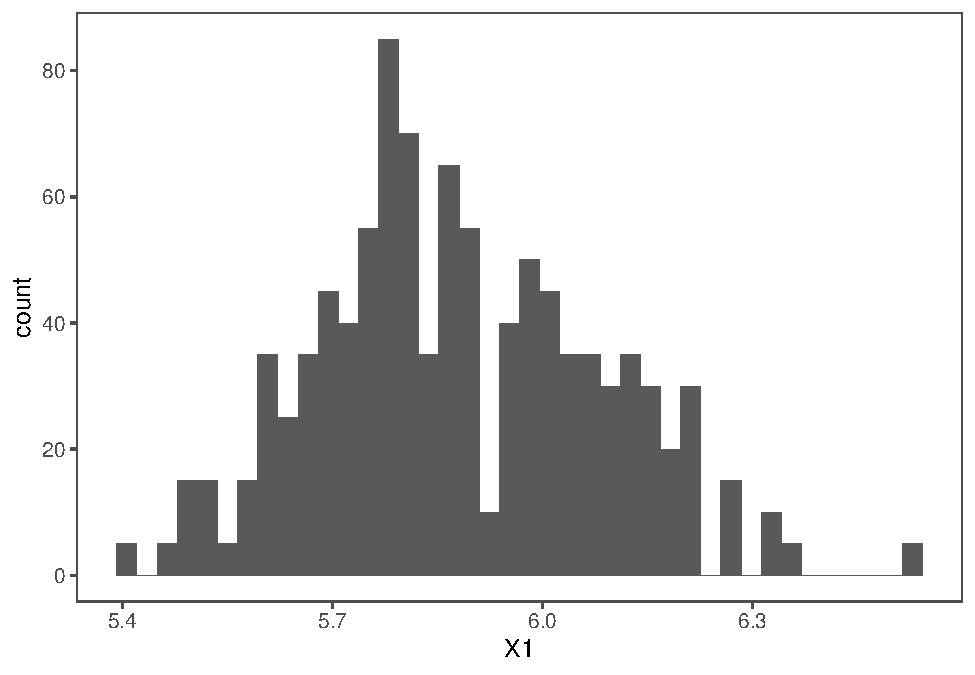
\includegraphics{Econo2_P4_files/figure-latex/mean ic-1} \end{center}

\begin{Shaded}
\begin{Highlighting}[]
\NormalTok{qq_x1 <-}\StringTok{ }\KeywordTok{qqnorm}\NormalTok{(fc_mean}\OperatorTok{$}\NormalTok{X1)}
\KeywordTok{qqline}\NormalTok{(fc_mean}\OperatorTok{$}\NormalTok{X1)}
\end{Highlighting}
\end{Shaded}

\begin{center}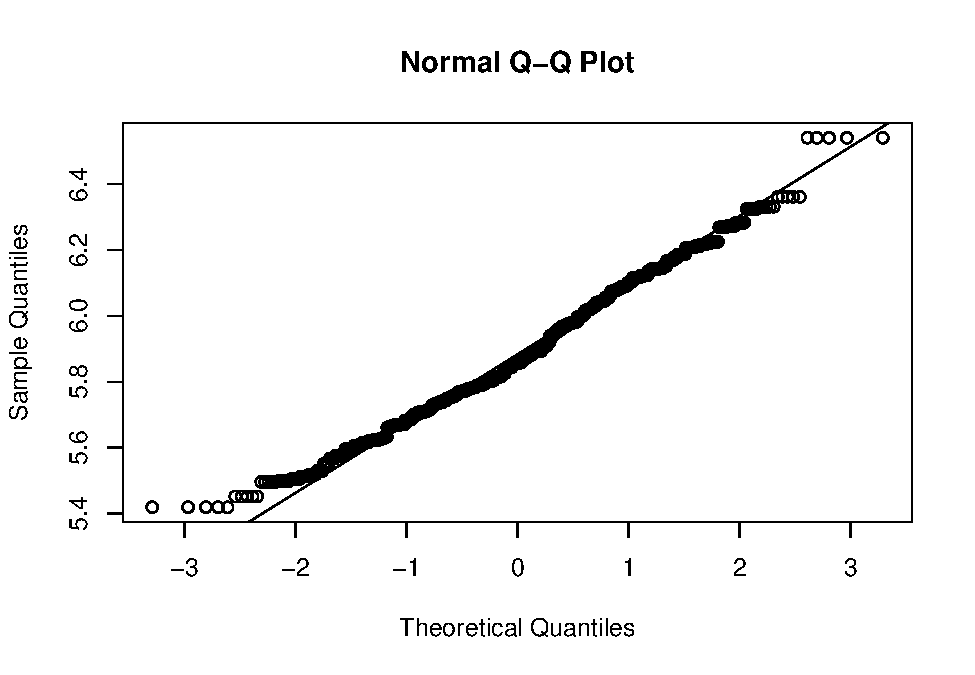
\includegraphics{Econo2_P4_files/figure-latex/mean ic-2} \end{center}

\begin{Shaded}
\begin{Highlighting}[]
\NormalTok{hist_x2 <-}\StringTok{ }\KeywordTok{ggplot}\NormalTok{(}\DataTypeTok{data =}\NormalTok{ fc_mean, }\KeywordTok{aes}\NormalTok{(}\DataTypeTok{x =}\NormalTok{ X2)) }\OperatorTok{+}\StringTok{ }\KeywordTok{geom_histogram}\NormalTok{(}\DataTypeTok{bins =} \DecValTok{40}\NormalTok{) }\OperatorTok{+}\StringTok{ }
\StringTok{    }\KeywordTok{theme_few}\NormalTok{()}
\NormalTok{hist_x2}
\end{Highlighting}
\end{Shaded}

\begin{center}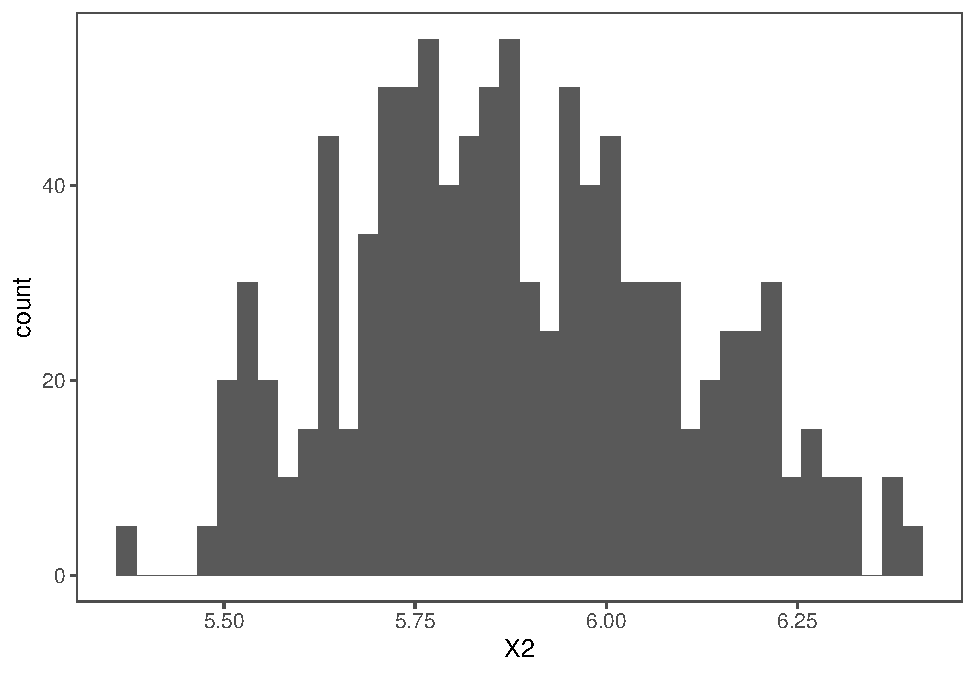
\includegraphics{Econo2_P4_files/figure-latex/mean ic-3} \end{center}

\begin{Shaded}
\begin{Highlighting}[]
\NormalTok{qq_x2 <-}\StringTok{ }\KeywordTok{qqnorm}\NormalTok{(fc_mean}\OperatorTok{$}\NormalTok{X2)}
\KeywordTok{qqline}\NormalTok{(fc_mean}\OperatorTok{$}\NormalTok{X2)}
\end{Highlighting}
\end{Shaded}

\begin{center}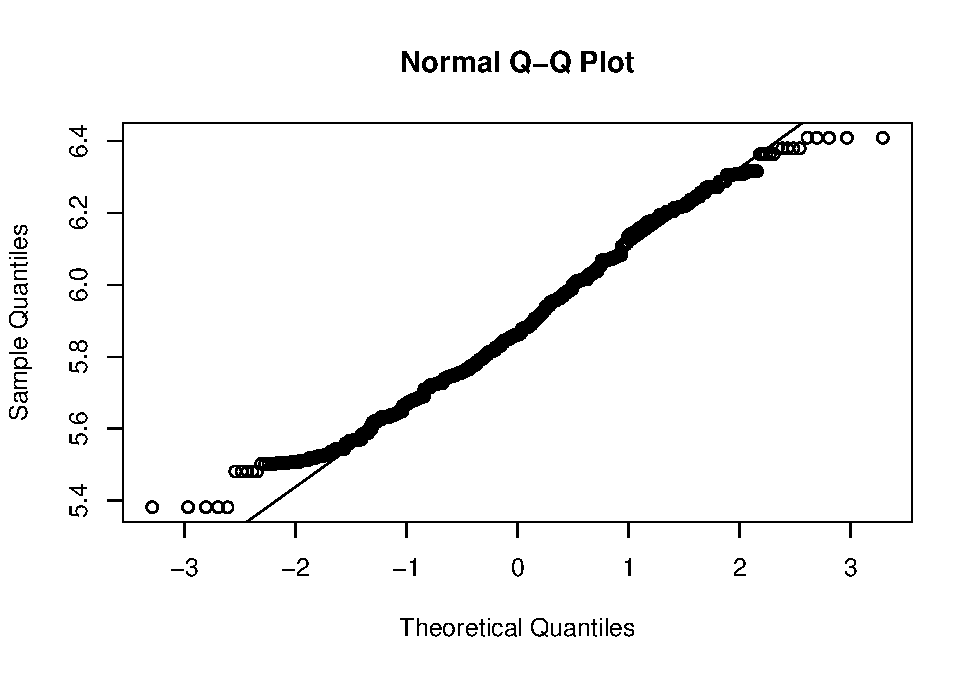
\includegraphics{Econo2_P4_files/figure-latex/mean ic-4} \end{center}

\begin{Shaded}
\begin{Highlighting}[]
\NormalTok{hist_x3 <-}\StringTok{ }\KeywordTok{ggplot}\NormalTok{(}\DataTypeTok{data =}\NormalTok{ fc_mean, }\KeywordTok{aes}\NormalTok{(}\DataTypeTok{x =}\NormalTok{ X3)) }\OperatorTok{+}\StringTok{ }\KeywordTok{geom_histogram}\NormalTok{(}\DataTypeTok{bins =} \DecValTok{40}\NormalTok{) }\OperatorTok{+}\StringTok{ }
\StringTok{    }\KeywordTok{theme_few}\NormalTok{()}
\NormalTok{hist_x3}
\end{Highlighting}
\end{Shaded}

\begin{center}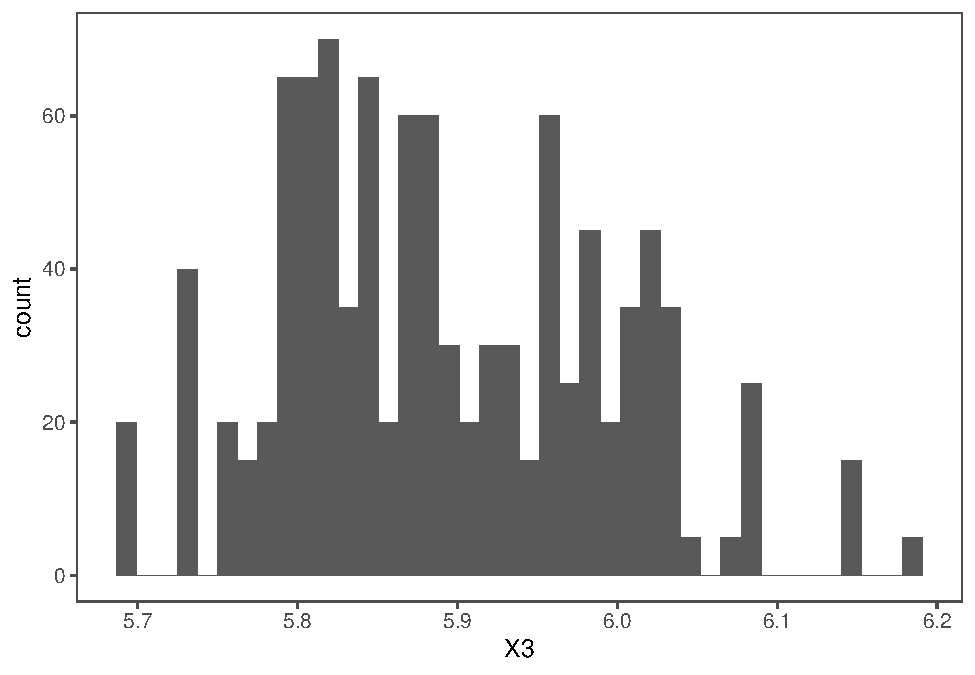
\includegraphics{Econo2_P4_files/figure-latex/mean ic-5} \end{center}

\begin{Shaded}
\begin{Highlighting}[]
\NormalTok{qq_x3 <-}\StringTok{ }\KeywordTok{qqnorm}\NormalTok{(fc_mean}\OperatorTok{$}\NormalTok{X3)}
\KeywordTok{qqline}\NormalTok{(fc_mean}\OperatorTok{$}\NormalTok{X3)}
\end{Highlighting}
\end{Shaded}

\begin{center}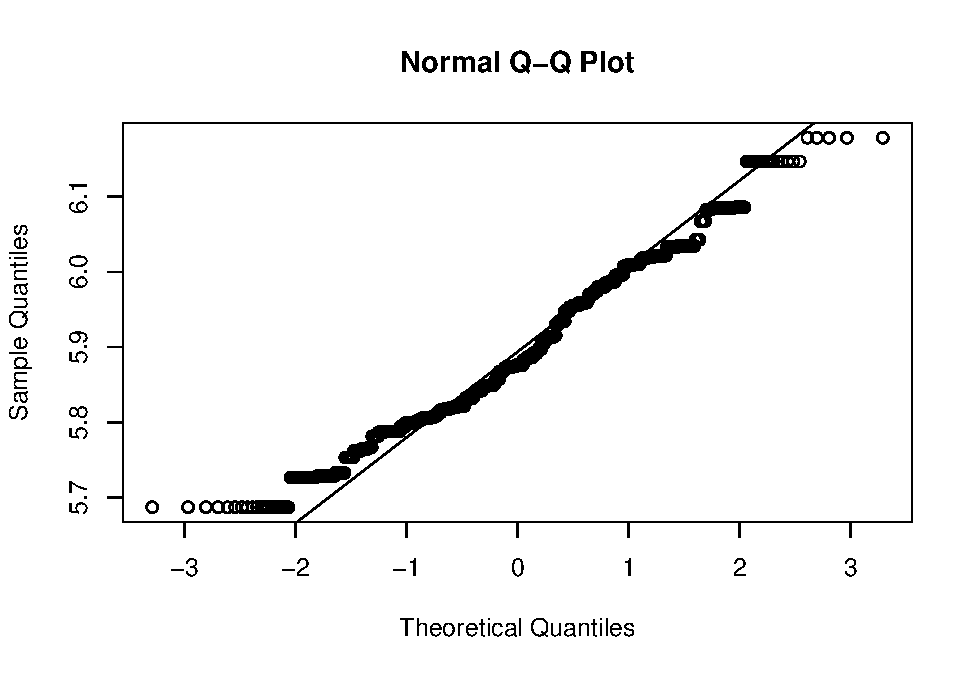
\includegraphics{Econo2_P4_files/figure-latex/mean ic-6} \end{center}

\begin{Shaded}
\begin{Highlighting}[]
\NormalTok{hist_x4 <-}\StringTok{ }\KeywordTok{ggplot}\NormalTok{(}\DataTypeTok{data =}\NormalTok{ fc_mean, }\KeywordTok{aes}\NormalTok{(}\DataTypeTok{x =}\NormalTok{ X4)) }\OperatorTok{+}\StringTok{ }\KeywordTok{geom_histogram}\NormalTok{(}\DataTypeTok{bins =} \DecValTok{40}\NormalTok{) }\OperatorTok{+}\StringTok{ }
\StringTok{    }\KeywordTok{theme_few}\NormalTok{()}
\NormalTok{hist_x4}
\end{Highlighting}
\end{Shaded}

\begin{center}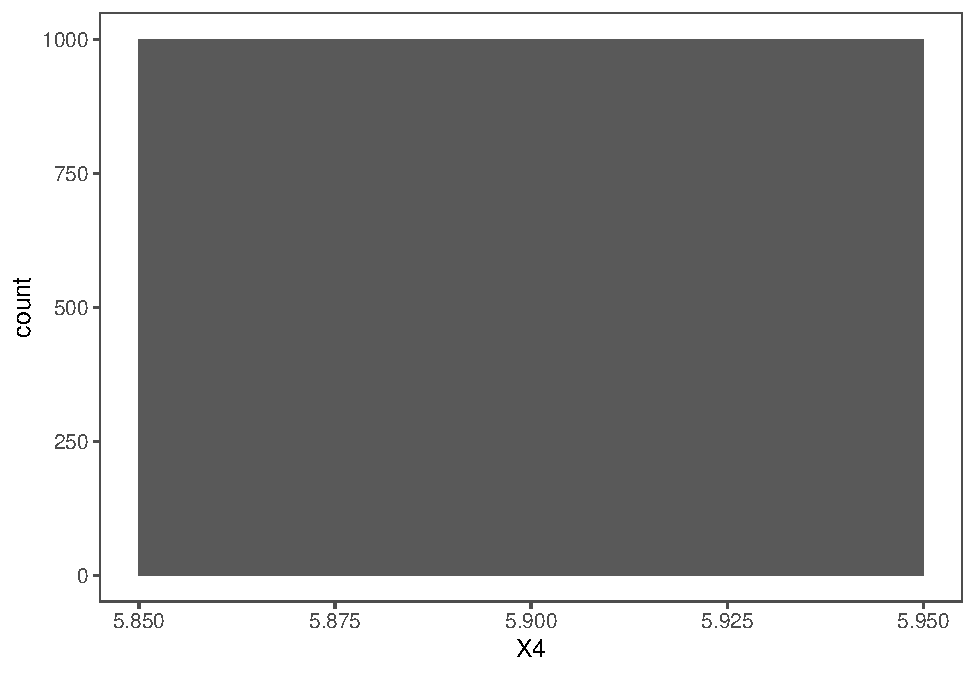
\includegraphics{Econo2_P4_files/figure-latex/mean ic-7} \end{center}

\begin{Shaded}
\begin{Highlighting}[]
\NormalTok{qq_x4 <-}\StringTok{ }\KeywordTok{qqnorm}\NormalTok{(fc_mean}\OperatorTok{$}\NormalTok{X4)}
\KeywordTok{qqline}\NormalTok{(fc_mean}\OperatorTok{$}\NormalTok{X4)}
\end{Highlighting}
\end{Shaded}

\begin{center}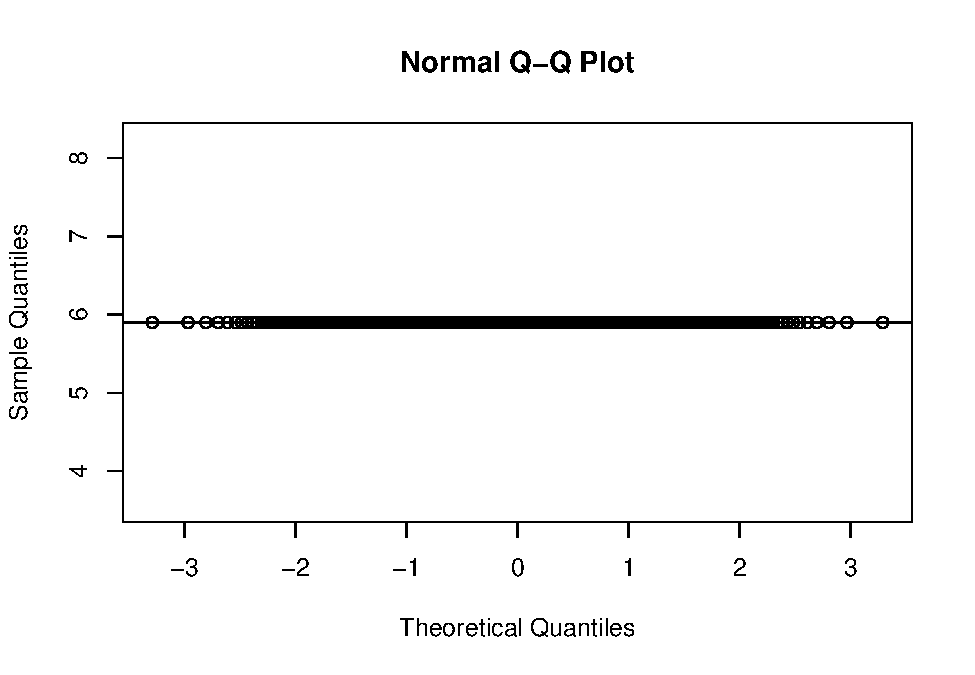
\includegraphics{Econo2_P4_files/figure-latex/mean ic-8} \end{center}

\begin{Shaded}
\begin{Highlighting}[]
\NormalTok{hist_x5 <-}\StringTok{ }\KeywordTok{ggplot}\NormalTok{(}\DataTypeTok{data =}\NormalTok{ fc_mean, }\KeywordTok{aes}\NormalTok{(}\DataTypeTok{x =}\NormalTok{ X5)) }\OperatorTok{+}\StringTok{ }\KeywordTok{geom_histogram}\NormalTok{(}\DataTypeTok{bins =} \DecValTok{100}\NormalTok{) }\OperatorTok{+}\StringTok{ }
\StringTok{    }\KeywordTok{theme_few}\NormalTok{()}
\NormalTok{hist_x5}
\end{Highlighting}
\end{Shaded}

\begin{center}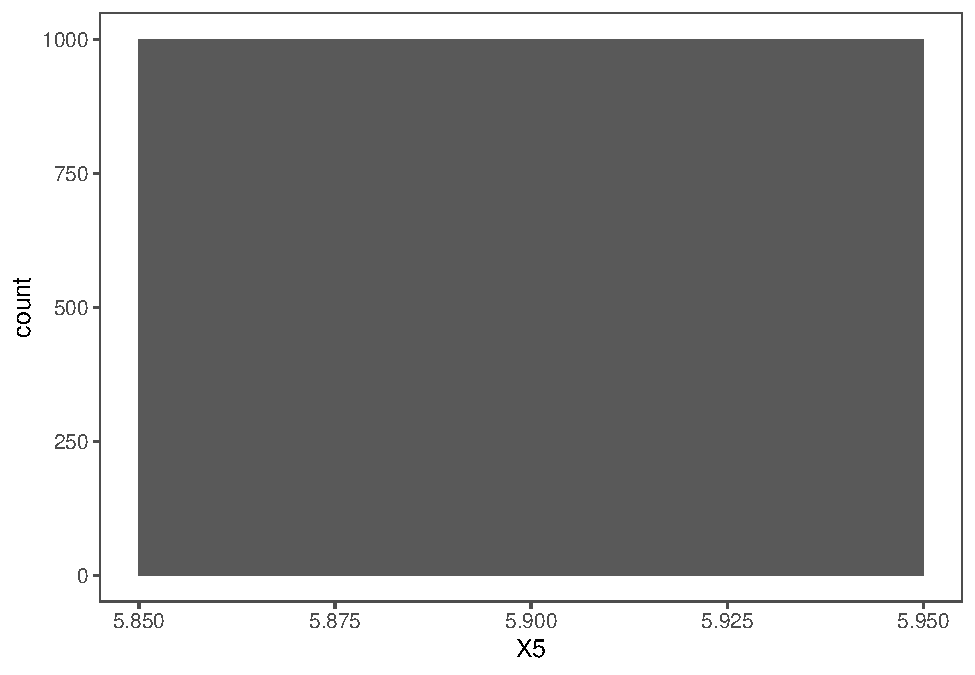
\includegraphics{Econo2_P4_files/figure-latex/mean ic-9} \end{center}

\begin{Shaded}
\begin{Highlighting}[]
\NormalTok{qq_x5 <-}\StringTok{ }\KeywordTok{qqnorm}\NormalTok{(fc_mean}\OperatorTok{$}\NormalTok{X5)}
\KeywordTok{qqline}\NormalTok{(fc_mean}\OperatorTok{$}\NormalTok{X5)}
\end{Highlighting}
\end{Shaded}

\begin{center}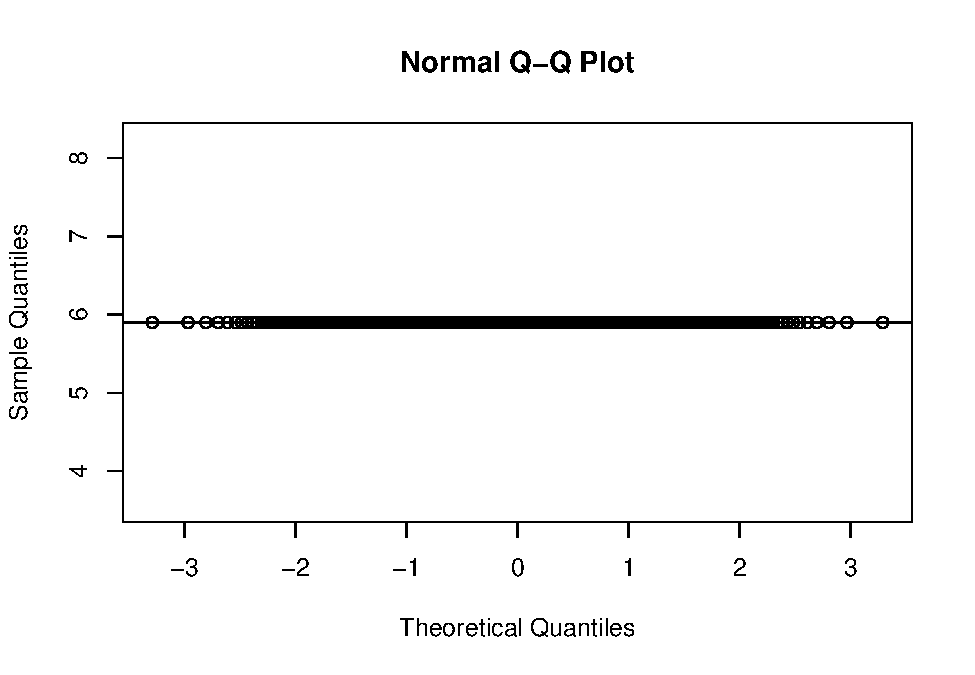
\includegraphics{Econo2_P4_files/figure-latex/mean ic-10} \end{center}

The results show that, from \(h \geq 4\), the predicted value is the
mean of the series.

Now, some forecasting plots:

\begin{Shaded}
\begin{Highlighting}[]
\NormalTok{fc <-}\StringTok{ }\KeywordTok{forecast}\NormalTok{(df}\OperatorTok{$}\NormalTok{value, }\DataTypeTok{model =}\NormalTok{ aa_model, }\DataTypeTok{h =}\NormalTok{ h)}

\KeywordTok{autoplot}\NormalTok{(fc) }\OperatorTok{+}\StringTok{ }\KeywordTok{theme_few}\NormalTok{()}
\end{Highlighting}
\end{Shaded}

\begin{center}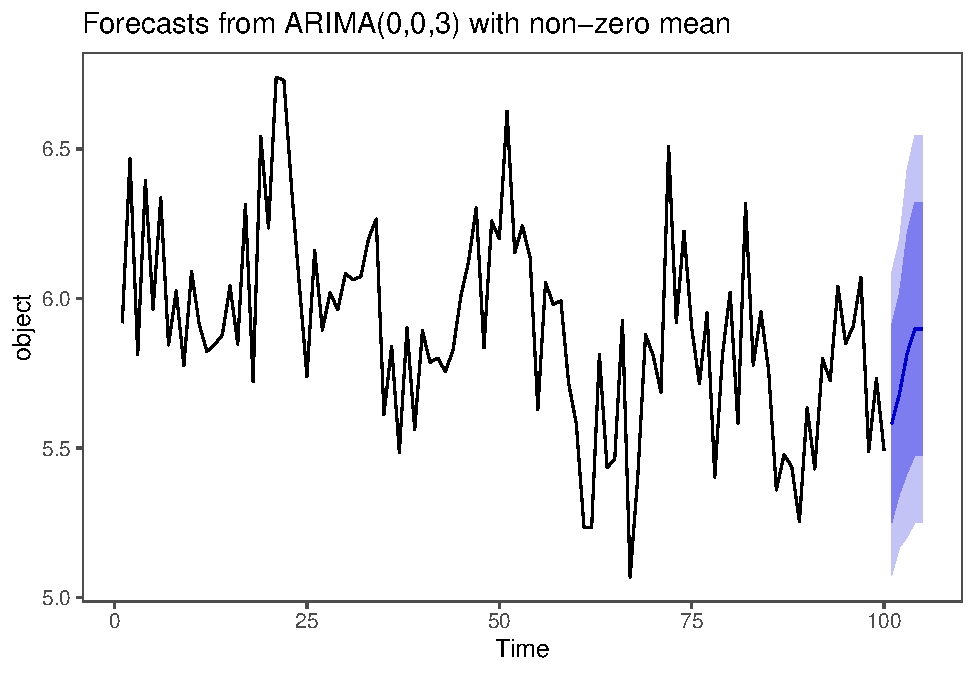
\includegraphics{Econo2_P4_files/figure-latex/forecast arima plots-1} \end{center}

\begin{Shaded}
\begin{Highlighting}[]
\KeywordTok{autoplot}\NormalTok{(fc_list[[}\DecValTok{1}\NormalTok{]]) }\OperatorTok{+}\StringTok{ }\KeywordTok{theme_few}\NormalTok{()}
\end{Highlighting}
\end{Shaded}

\begin{center}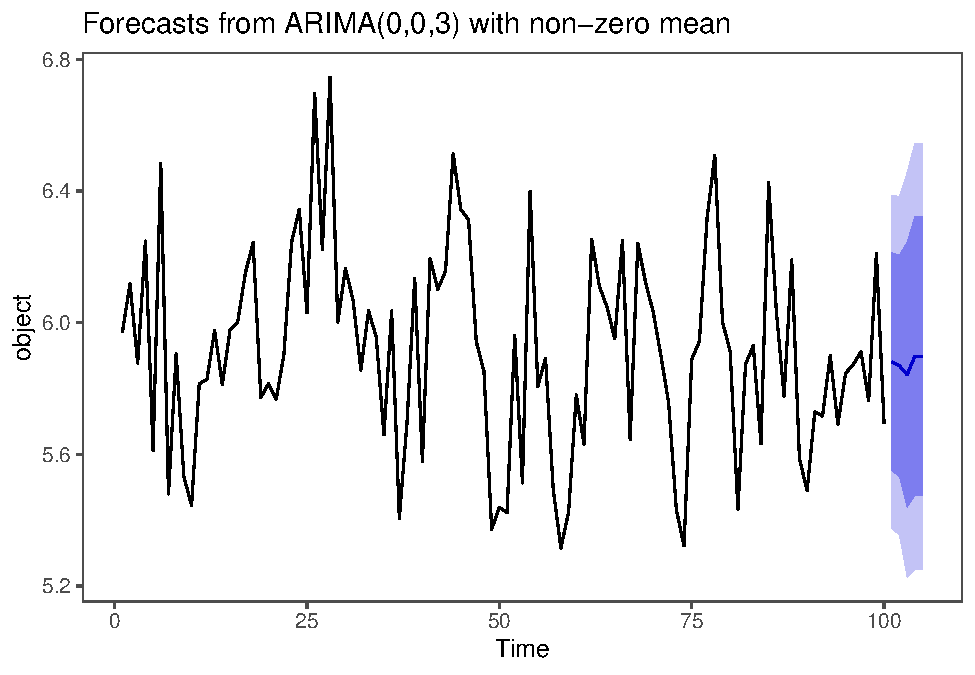
\includegraphics{Econo2_P4_files/figure-latex/forecast arima plots-2} \end{center}

\begin{Shaded}
\begin{Highlighting}[]
\KeywordTok{autoplot}\NormalTok{(fc_list[[}\DecValTok{66}\NormalTok{]]) }\OperatorTok{+}\StringTok{ }\KeywordTok{theme_few}\NormalTok{()}
\end{Highlighting}
\end{Shaded}

\begin{center}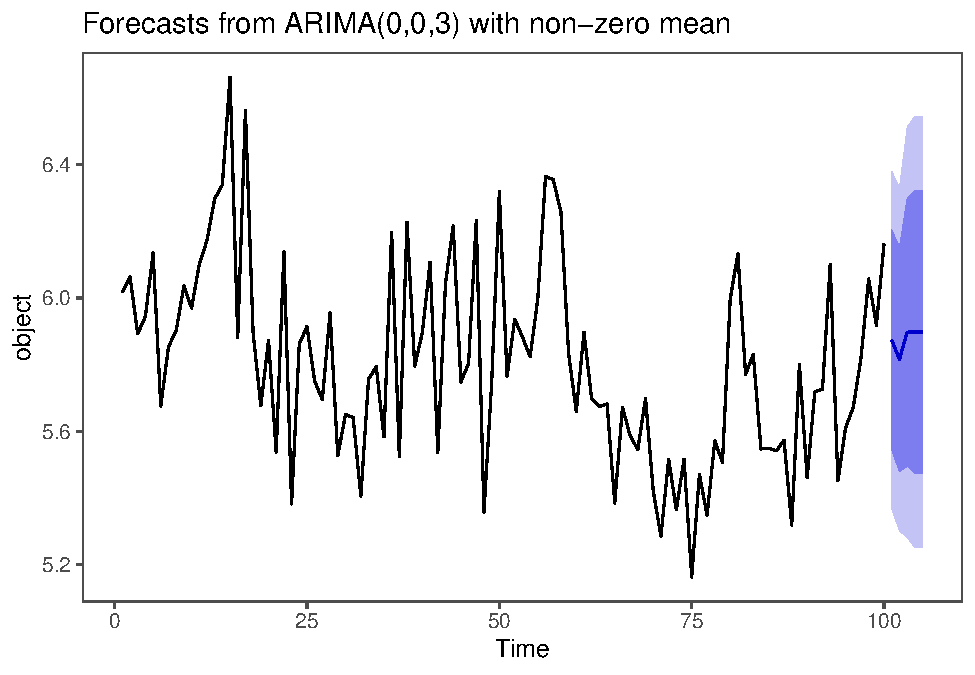
\includegraphics{Econo2_P4_files/figure-latex/forecast arima plots-3} \end{center}

\begin{Shaded}
\begin{Highlighting}[]
\KeywordTok{autoplot}\NormalTok{(fc_list[[}\DecValTok{796}\NormalTok{]]) }\OperatorTok{+}\StringTok{ }\KeywordTok{theme_few}\NormalTok{()}
\end{Highlighting}
\end{Shaded}

\begin{center}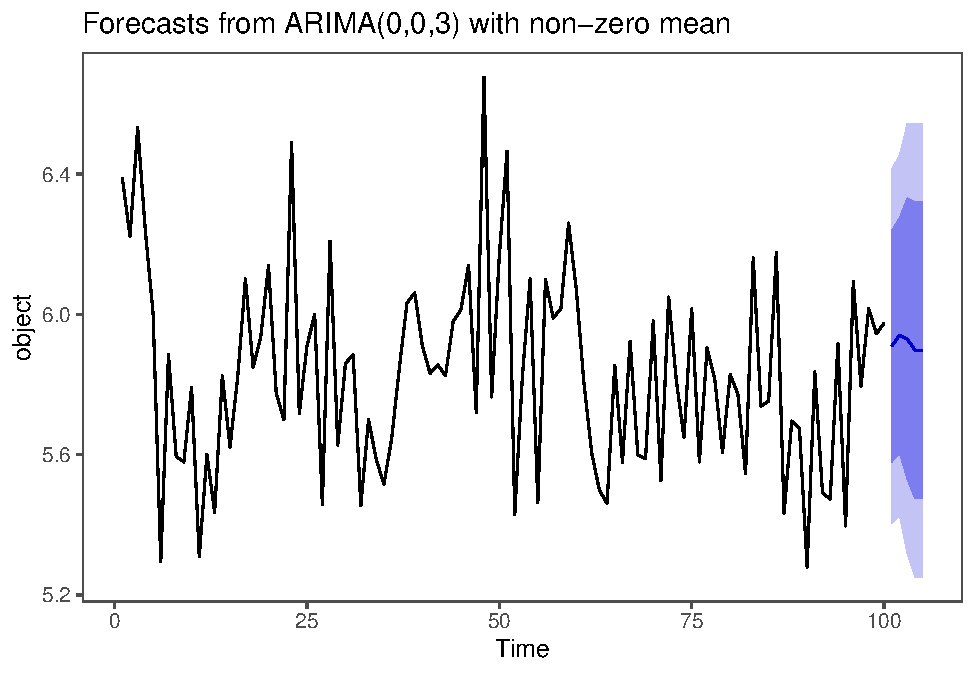
\includegraphics{Econo2_P4_files/figure-latex/forecast arima plots-4} \end{center}

\end{document}
